\documentclass[a4paper, oneside, 12pt]{article}
\usepackage{fancyhdr}  
\usepackage[]{geometry}
\usepackage{verbatim}
\usepackage[T1]{fontenc}
\usepackage[utf8]{inputenc}
\usepackage{csquotes}
\usepackage[swedish]{babel}
\usepackage{tabularx, booktabs}
\usepackage{lmodern}
\usepackage{hyperref}
\usepackage{float}
\usepackage{subfiles}
\usepackage{titlesec}
\usepackage{titling}
\usepackage{graphicx,wrapfig,lipsum}
\usepackage{gensymb}
\usepackage{siunitx}
\usepackage{tocloft}
\usepackage{listings}
\usepackage{xcolor}
\usepackage{color}
\usepackage[linesnumbered,ruled,vlined]{algorithm2e}
%\usepackage{biblatex}
\usepackage{amsmath}
%\addbibresource{ref.bib}
 
%============================> NEW COMMANDS <==================================
%TODO: Define these vars
\newcommand{\courseName}{COURSE NAME}
\newcommand{\courseCode}{COURSE CODE}
\newcommand{\assignmentName}{ASSIGNMENT NAME}
\newcommand{\courseStaff}{Someone ,  Someone , Someone}


\newcommand{\subtitle}[1]{%
	\posttitle{%
	\par\end{center}
	\begin{center}\normalsize#1\end{center}
	\vskip0.5em}%
}



%============================> STYLINGS <=====================================

\definecolor{codegreen}{rgb}{0,0.6,0}
\definecolor{codegray}{rgb}{0.5,0.5,0.5}
\definecolor{codepurple}{rgb}{0.58,0,0.82}
\definecolor{backcolour}{rgb}{0.95,0.95,0.92}
 
\lstdefinestyle{mystyle}{
    backgroundcolor=\color{backcolour},   
    commentstyle=\color{codegreen},
    keywordstyle=\color{magenta},
    numberstyle=\tiny\color{codegray},
    stringstyle=\color{codepurple},
    basicstyle=\footnotesize,
    breakatwhitespace=false,         
    breaklines=true,                 
    captionpos=b,                    
    numbers=left,                    
    numbersep=4pt,                  
    showspaces=false,                
    showstringspaces=false,
    showtabs=false,                  
    tabsize=1,
   % keepspaces=true             
}
%\renewcommand{\headrulewidth}{}



%============================>  SETTINGS <=====================================
%TODO: clean this!! 
\lstset{style=mystyle}
\hypersetup{colorlinks=true, linkcolor=black}
\pagestyle{fancy}
\fancyhf{}


\graphicspath{ {image/} }
\setlength\parindent{0pt}
\setlength{\parskip}{0.8em}


\begin{document}

\title{\courseName \\ \courseCode } 
\subtitle{\assignmentName} 
\author{\\ \\ \LARGE Abdulsalam Aldahir \\   dv18aar@cs.umu.se}
\date{\today}


\begin{titlepage}
\maketitle 
\thispagestyle{fancy}
\headheight 35pt
\rhead{\small\today}
\lhead{\small Umeå universitet \\ Institutionen för datavetenskap }
\vspace{3cm}\hspace{4cm}


\cfoot{\courseName \\ \courseStaff \\}

\end{titlepage}

% Table of Contents
\pagenumbering{roman}
\tableofcontents{}


\newpage
\pagestyle{fancy}
\fancyhf{}
\rhead{\today}
\lhead{ Abdulsalam Aldahir \\ dv18aar@cs.umu.se}
\cfoot{\thepage}  
%\hypersetup{colorlinks=true,urlcolor=blue,urlbordercolor={0 1 1}}
\clearpage
\pagenumbering{arabic}
\setcounter{page}{1}


\section{Introduction}

\section{Background}

\section{Method}
  

\begin{align}
\label{MM}
	max_{j\in [0..n]}
 \begin{cases}
	 maxJ(j)
 \end{cases}
\end{align}

\begin{align}
\label{MM_2}
	maxJ(j) = max
 \begin{cases}
	 CC(j) + RR(n-j) \\
	 DD(j) + SS(n-j) - G_{open} \\
 \end{cases}
\end{align}




\section{Results}
\begin{figure}[H]
    \centering
    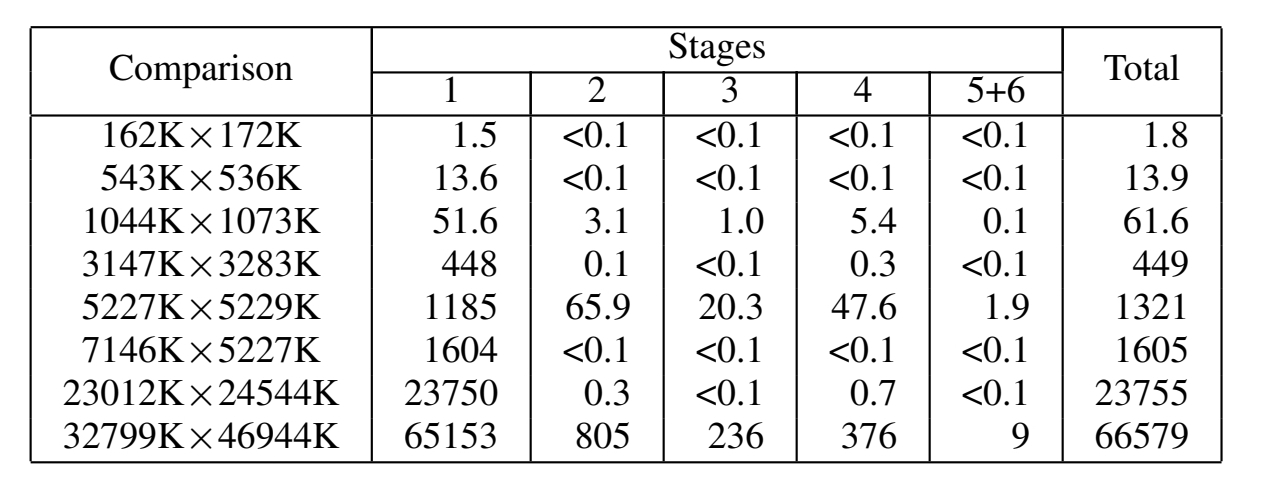
\includegraphics[height=1.5in]{image/runTime_stages.jpg}
    \caption{The Speed up results of the algorithm\cite{cuda2}}
    \label{fig:cuda2_stages}
\end{figure}

\section{Discussion}





\newpage


\bibliographystyle{plain}
\bibliography{reference}

\end{document}
